\documentclass[../main.tex]{subfiles}

\begin{document}

\chapter{Soft Tissue Engineering}

\section{Stress \& strain in large deformations}

\subsection{Kinematics}

\begin{itemize}
    \item Mapping function 
    \begin{align}
        \vec{x} = \underline{\varphi}(\vec{X},t)
    \end{align}
    \item Displacement function
    \begin{align}
        \vec{x} = \vec{X} + \underline{U}(\vec{X},t)
    \end{align}
    \item The deformation gradient tensor
    \begin{align}
        d\vec{x} = \textbf{F}(X,t)d\vec{X} \Rightarrow \textbf{F} = \frac{\partial \vec{x}}{\partial \vec{X}} = \frac{\partial \underline{\varphi}}{\partial \vec{X}}
    \end{align}
    \item Volume transformation
    \begin{align}
        dv = \det(\textbf{F})dV=JdV
    \end{align}
    \item Surface transformation: Nanson's Formula
    \begin{align}
        \vec{n}ds = J\textbf{F}^{-\top}\vec{N}dS
    \end{align}
    \item Polar decomposition
    \begin{align}
        \textbf{F} = \textbf{R}\textbf{U} = \textbf{V}\textbf{R} \\
        \Rightarrow \textbf{U}^2 = \textbf{F}^{\top}\textbf{F} = \textbf{C}\\
        \Rightarrow \textbf{V}^2 = \textbf{F}\textbf{F}^{\top} = \textbf{B}
    \end{align}
\end{itemize}

\subsection{Strain}

\begin{itemize}
    \item Nominal strain, Biot strain or Engineering strain
    \begin{align}
        \textbf{e} = \textbf{U} - \textbf{I}
    \end{align}
    \item Green-Lagrange strain
    \begin{align}
        \textbf{E} = \frac{1}{2}(\textbf{F}^{\top}\textbf{F} - \textbf{I}) = \frac{1}{2}(\textbf{U}^2 - \textbf{I})
    \end{align}
    \item Euler-Almansi strain
    \begin{align}
        \textbf{A} = \frac{1}{2}(\textbf{I}-\textbf{V}^{-2})
    \end{align}
    \item True strain or logarithmic strain
    \begin{align}
        \bm{\varepsilon} = \ln(\textbf{U})
    \end{align}
\end{itemize}

\subsection{Stress}

\begin{itemize}
    \item True stress or Cauchy stress
    \begin{align}
        \bm{\sigma}^{\top} = \frac{d\vec{f}}{\vec{n}dS}
    \end{align}
    \item 1PK: first Piola Kirchoff stress (Nominal stress or Engineering stress)
    \begin{align}
        \textbf{P} = \frac{d\vec{f}}{\vec{N}dS_0}
    \end{align}
    \item 2PK: second Piola Kirchoff stress
    \begin{align}
        \textbf{S}^{\top} = \frac{\textbf{F}^{-1}d\vec{f}}{\vec{N}dS_0}
    \end{align}
    \item Swithcing between stresses:
    \begingroup
        %\setlength{\tabcolsep}{20pt}
        \renewcommand{\arraystretch}{1.5}
        \begin{tabular}{c|ccc}
             & $\bm{\sigma}$ & \textbf{P} & \textbf{S} \\
            \hline
            $\bm{\sigma}$ & $\bm{\sigma}$ & $J^{-1}\textbf{P}\textbf{F}^{\top}$ & $J^{-1}\textbf{F}\textbf{S}\textbf{F}^{\top}$\\
            \textbf{P} & $J\bm{\sigma}\textbf{F}^{\top}$ & \textbf{P} & \textbf{F}\textbf{S}\\
            \textbf{S} & $J\textbf{F}^{-1}\bm{\sigma}\textbf{F}^{-\top}$ & $\textbf{F}^{-1}\textbf{P}$ & \textbf{S} \\
        \end{tabular}
    \endgroup
\end{itemize}

\section{Constitutive modeling}

\section{Mechanical testing \& parameter fitting}

\subsection{Uniaxial tensile testing}

\subsection{Biaxial tensile testing}
\subsection{Extenson-inflation testing}
\subsection{Strain mapping}

\section{In vivi wall stress estimation}

\subsection{Laplace's law for thin-walled tubes}

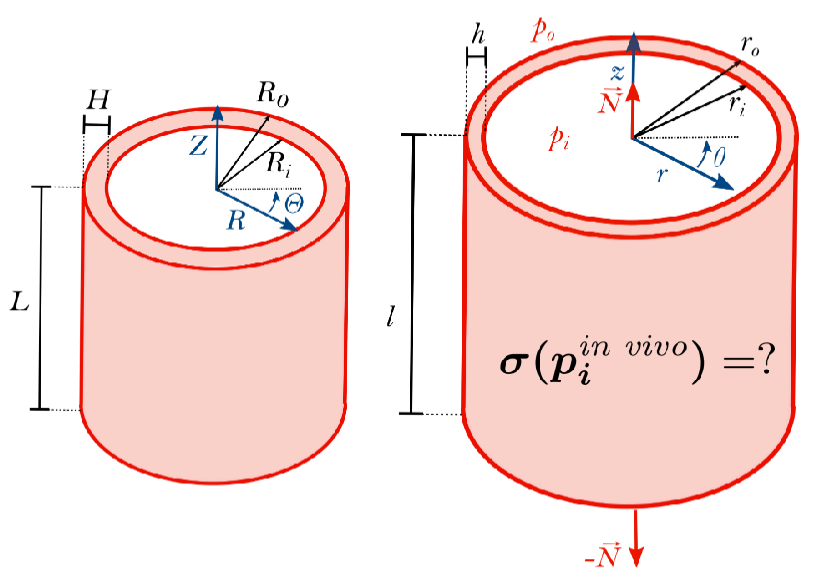
\includegraphics[scale=0.5]{cylindricaltissue.png}

The deformation gradient tensor is givan as
\begin{align}
    \textbf{F} = \left[\begin{matrix}
        1/(\lambda_{\theta}\lambda_z) & 0 & 0 \\
        0 & \lambda_{\theta} & 0 \\
        0 & 0 & \lambda_z
    \end{matrix}\right]
\end{align}
with corresponding stresses
\begin{align}
    \langle \sigma_{rr} \rangle &= -\frac{P}{2} \\
    \langle \sigma_{\theta\theta} \rangle &= \frac{P}{h/r_i}\\
    \langle \sigma_{zz} \rangle &= \frac{||\vec{N}||}{\pi(r^2_0-r^2_i)}
\end{align}
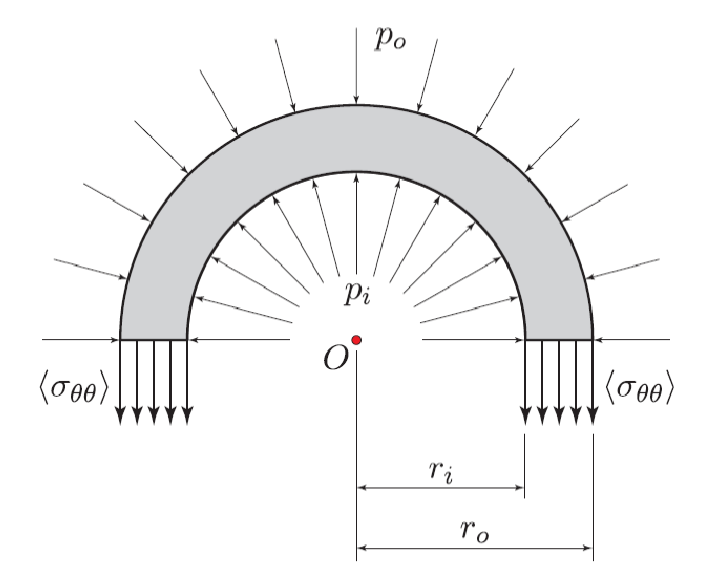
\includegraphics[scale=0.5]{cylindricaltissueslice.png}

\subsection{Analytical analysis fot thick-walled cylinders}

\subsection{The Finite Element Method}

\section{Other biomechanical applications}

\end{document}